\chapter{Task 28: Voter Model}

\section{Task Description}
The voter model is perhaps the simplest and most studied model of cooperative behaviour. While its behaviour on regular lattices of arbitrary dimension $d$ is known in detail, it is much more difficult to get a comprehensive general picture of its behaviour on a complex network, where there is interplay between many factors, such as degree distribution, correlations, effective dimensionality and level of disorder\cite{suchecki_numerical}. 
The aim of this task is to describe the voter model and attempt to reproduce its behaviour on some class of networks. Specifically, I chose to focus on scale free networks, for which some analitical results have been found \cite{sood}. 

\section{Mathematical Model}
In the voter model, each node of the network is in one of two possible states $\sigma_i \in \{\pm 1\}$ (say, for instance, spin up or down). The evolution starts with some random configuration of up and down spins. The update rule is defined as follows: 
\medskip
\newline
\begin{minipage}{0.8\textwidth}
\begin{itemize}
    \item[i)] choose one node at random,
    \item[ii)] choose one of its neighbors at random,
    \item[iii)] ascribe to this node the current state of its neighbour.
\end{itemize}
\end{minipage}
\hfill
\begin{minipage}{0.2\textwidth}
\vfill
    \textit{Node-update rule}
\vfill
\end{minipage}
\medskip
\newline
Actually, there is an alternative rule which may look equivalent:
\medskip
\newline
\begin{minipage}{0.8\textwidth}
\begin{itemize}
    \item[i)] choose one link at random,
    \item[ii)] choose one of its ends at random,
    \item[iii)] ascribe to this node end the current state of the other end.
\end{itemize}
\end{minipage}
\hfill
\begin{minipage}{0.2\textwidth}
\vfill
    \textit{Link-update rule}
\vfill
\end{minipage}
\medskip
\newline
At each time step, this update rule is applied $N$ times if $N$ is the network size, so that \textit{on average} each node is updated once. The two rules are equivalent for regular lattices, but not in the case of complex networks \cite{suchecki_analitical}. The voter model defines a markovian stochastic process. There are two absorbing states: all spins up and all spins down (they are called absorbing because when the system reaches one of these states, by the update rules it remains there forever). If we identify network nodes as people and spin up and down with two possible opinion, the absorbing states represent unanimous consensus. \\
There is always a chance that a finite size network reaches consensus. In fact, \textbf{the mean time required to reach consensus in a finite network is always finite}, whether it is a regular lattice or a complex network.  The mean is intended here an ensemble mean, computed over the set of all evolution histories and all initial conditions. However, conceptually, there are different scenarios when infinite size networks are considered instead.\\
The mean time $\left \langle \tau \right \rangle$ to reach consensus in a finite, regular lattice of $N$ nodes and dimension $d$ is known to scale as:
\begin{equation*}
    \left \langle \tau \right \rangle(N) \sim
    \begin{cases}
        N^2 \quad &\text{if}\quad d=1 \\
        N\cdot \ln{N} &\text{if}\quad d=2 \\
        N &\text{if}\quad d>2 \\
    \end{cases}
\end{equation*}
For networks, one could guess that $\left \langle \tau \right \rangle(N) \sim N$ as happens for high dimensional lattices. However this is not true in general. For instance, \cite{sood} found analitically that, for uncorrelated, scale-free networks with degree distribution $P(k)\sim k^{-\gamma}$ and \textit{node-update} rule:
\begin{equation*}
    \left \langle \tau \right \rangle(N) \sim
        \begin{cases}
         N^{\alpha}, \, \alpha<1 \quad &\text{if}\quad \gamma < 3 \\
        \frac{N}{\ln{N}} &\text{if}\quad \gamma = 3 \\
         N &\text{if}\quad \gamma > 3 \\
    \end{cases}
\end{equation*}
Addiotionally, they found out numerically that also scale- free networks with degree-degree correlations align well with these formulas. The authors of \cite{suchecki_numerical} numerically found for Barabasi-Albert (BA) networks a scaling $\tau \sim N^{0.88}$, which is compatible with the theoretical prediction $\tau \sim \frac{N}{\ln{N}}$. Furthermore, they found that when the \textit{edge-update} rule is used instead, a scaling $\tau \sim N$ is found, which is the same as that of high dimensional lattices. \\
A standard order parameter used to measure the ordering process of the voter dynamic is the \textit{average interface density $\rho$}, defined as the density of edges connecting nodes with different states:
\begin{equation}
    \rho(\mathbf{\sigma}) := \frac{\sum_{i,\,j}\left[A_{i,\,j}\,\cdot \mathbbm{1}(\sigma_i,\,\sigma_j)\right]}{\sum_{i,\,j}\, A_{i,\,j}}, \quad \text{where} \, \mathbbm{1}(\sigma_i,\,\sigma_j):= \frac{1 - \sigma_i\,\sigma_j}{2} = 
    \begin{cases}
        1 & \text{if}\quad \sigma_i\neq \sigma_j \\
        0 & \text{if}\quad \sigma_i= \sigma_j \\
    \end{cases}
\label{eq:rho}
\end{equation}
The interface density $\rho$ measures the level of disorder present in the network, and is zero when consensus is reached. 
\section{Numerical Simulations}
For my simulation, I tried to verify the scaling law $\tau(N)\sim N\cdot\ln{N}$ on BA networks.
\begin{figure}[H]
    \centering
    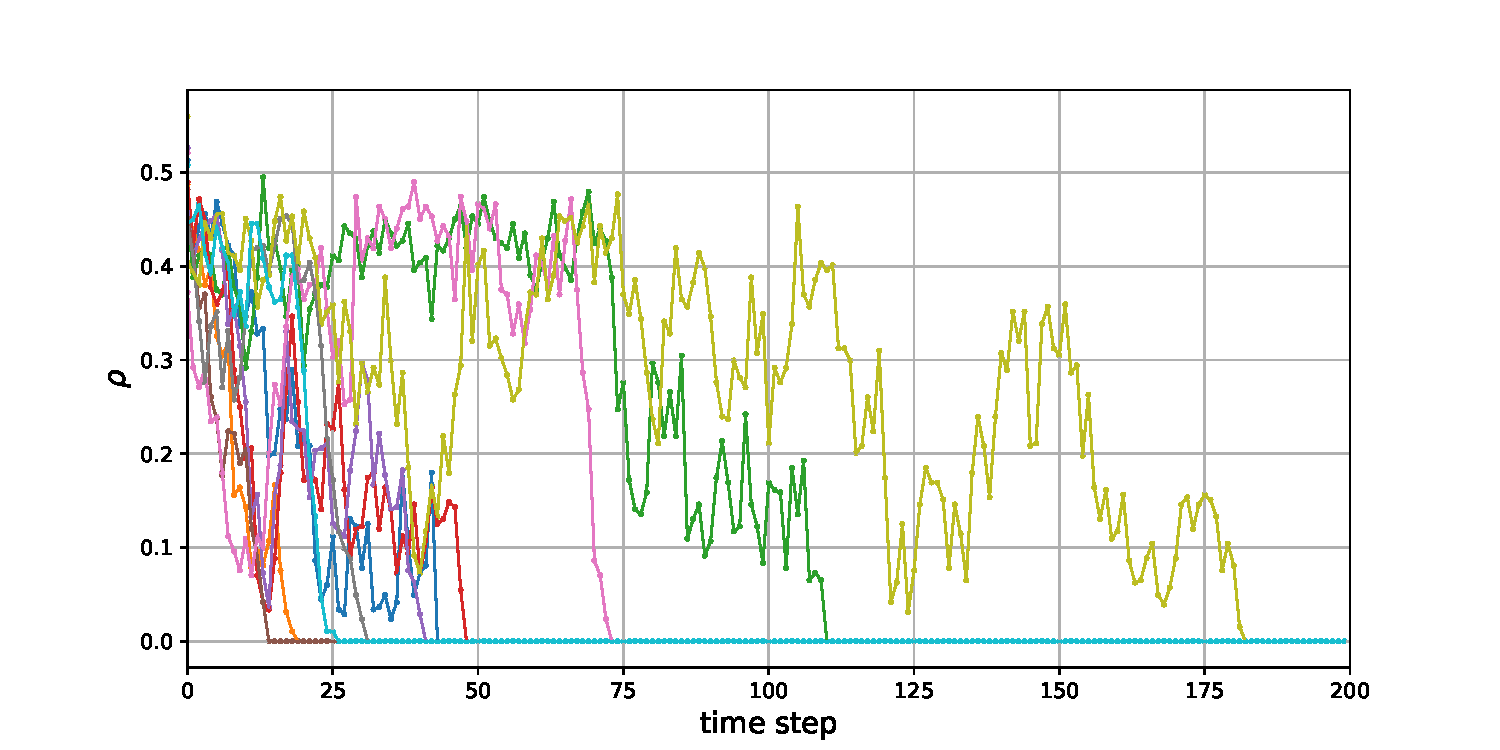
\includegraphics[width=0.8\linewidth]{latex_source/images/voter/example_evolution.pdf}
    \caption{Evolution of the voter model on Barabasi-Albert networks with $N=100$ and $\left\langle k\right\rangle = 8$. Each line is a trajectory on a different network instance. The initial state of each node is sampled with equal probability as $+1$ or $-1$.}
    \label{fig:enter-label}
\end{figure}

\begin{figure}[H]
    \centering
    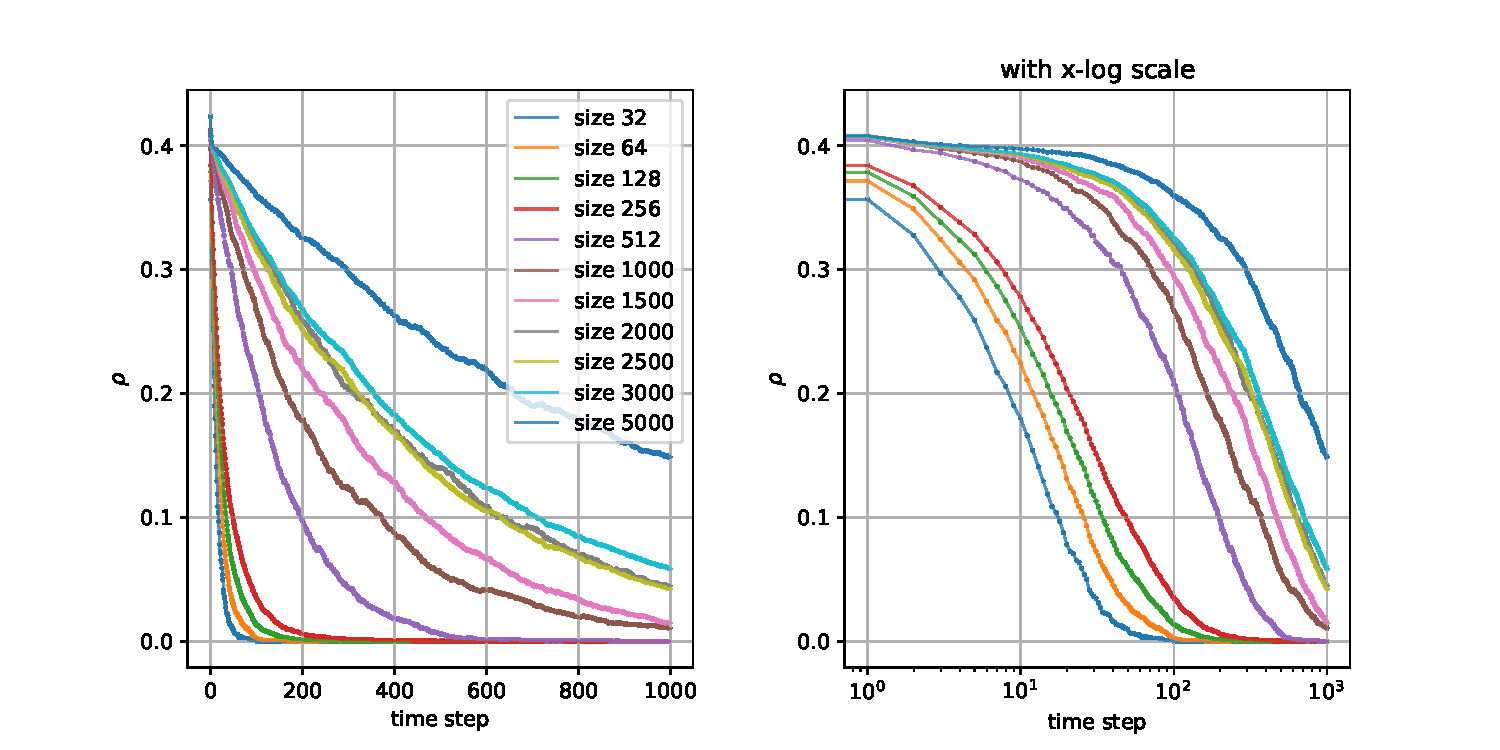
\includegraphics[width=\linewidth]{latex_source/images/voter/BA_node_update_rule_results_logscale.pdf}
    \caption{Evolution of the average interface density [Eq. $\ref{eq:rho}$] in Barabasi Albert networks of mean degree $\left\langle k\right\rangle= 6$ different sizes. Data is averaged over $500$ realizations. }
    \label{fig:BA_evolution}
\end{figure}

\begin{figure}[H]
    \centering
    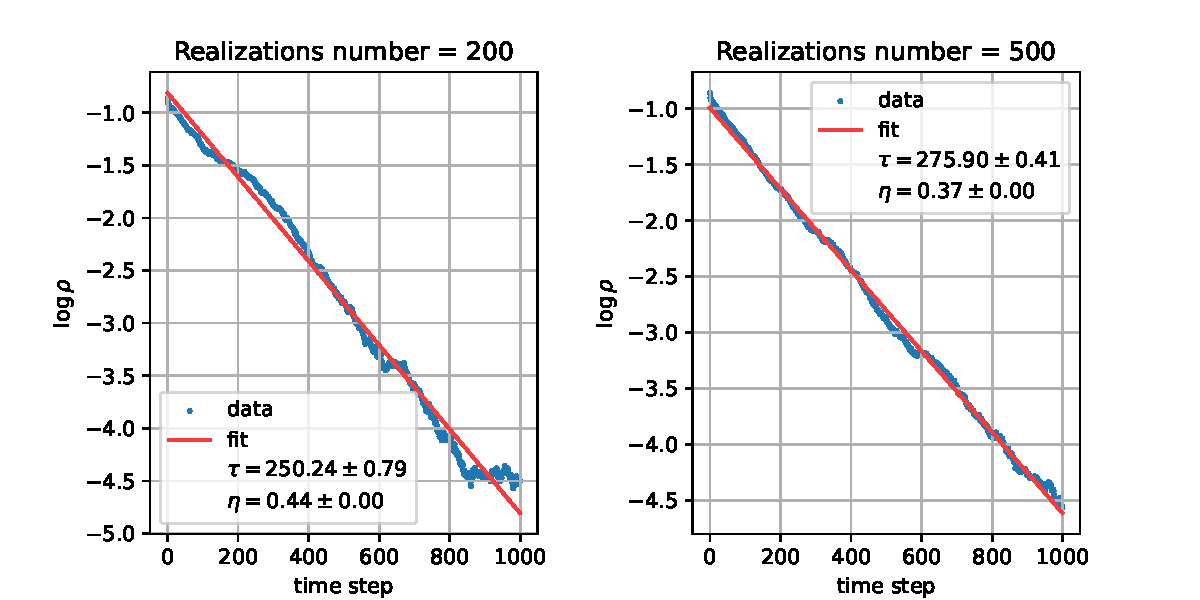
\includegraphics[width=\linewidth]{latex_source/images/voter/comparison.pdf}
    \caption{Comparison between exponential fit parameters estimated from $200$ (left) and $500$ (right) different realization on BA networks with same size $N=1000$. }
    \label{fig:enter-label}
\end{figure}

\begin{figure}[H]
    \centering
    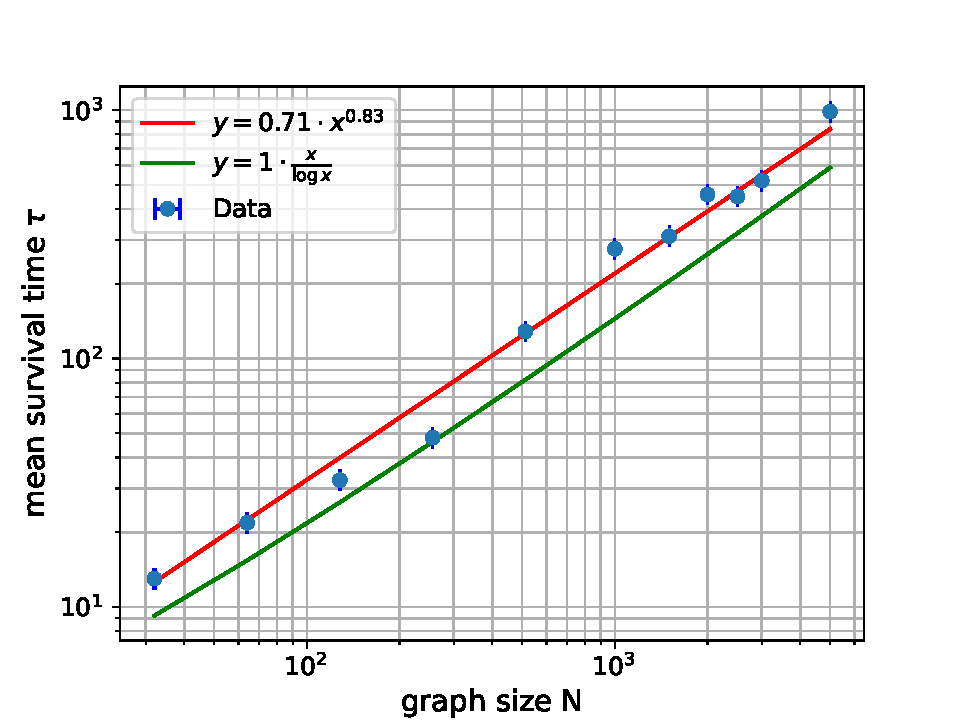
\includegraphics[width=0.7\linewidth]{latex_source/images/voter/BA_time_scaling.pdf}
    \caption{Average survival times for Barabasi Albert networks of different sizes, as results from the exponential fit of the curves in [Fig: $\ref{fig:BA_evolution}$]. Data is fitted with a power law $y = \alpha \cdot x^\gamma$ with free parameters $\alpha,\, \gamma$ with the method of least squares For comparison, also the theoretical expectation $\tau \sim \frac{N}{\log{N}}$ is plotted (green line). One can see that the slope of the two curves are very similar.}
    \label{fig:BA_scaling}
\end{figure}